%
% 2-jacobi.tex
%
% (c) 2021 Prof Dr Andreas Müller, OST Ostschweizer Fachhochschule
%
\section{Jacobische elliptische Funktionen
\label{buch:elliptisch:section:jacobi}}
\kopfrechts{Jacobische elliptische Funktionen}
Die elliptischen Integrale von
Abschnitt~\ref{buch:elliptisch:section:integral}
können dazu verwendet werden, die Länge eines Ellipsenbogens aus
den Koordinaten der Endpunkte zu berechnen.
Die trigonometrischen Funktionen drücken dagegen umgekehrt die
Koordinaten eines Punktes auf einem Kreis aus der Länge des
Kreisbogens aus.
Das elliptische Integral, welches die Bogenlänge auf einer Ellipse zwischen
den Punkten $(1,0)$ und $(x,y)$ entsprecht also eher der Funktion
$\arcsin y=\sin^{-1}y$.
Möchte man Funktionen konstruieren, die die Eigenschaften der 
trigonometrischen Funktionen auf die Geometrie von Ellipsen erweitern,
dann muss man die Umkehrfunktionen der elliptischen Integrale dafür ins
Auge fassen.

%
% elltrigo.tex
%
% (c) 2022 Prof Dr Andreas Müller, OST Ostschweizer Fachhochschule
%

%
% elliptische Funktionen als Trigonometrie
%
\subsection{Elliptische Funktionen als Trigonometrie}
\begin{figure}
\centering
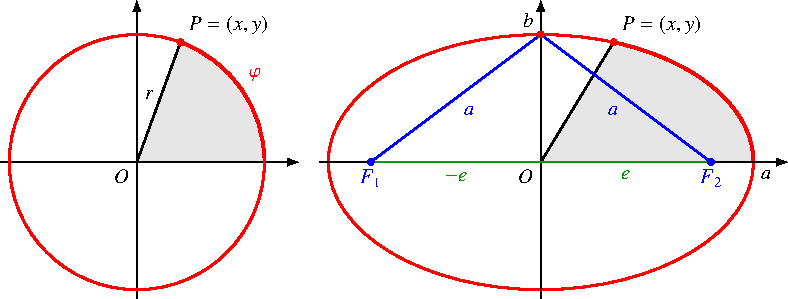
\includegraphics{chapters/110-elliptisch/images/ellipse.pdf}
\caption{Kreis und Ellipse zum Vergleich und zur Herleitung der 
elliptischen Funktionen von Jacobi als ``trigonometrische'' Funktionen
auf einer Ellipse.
\label{buch:elliptisch:fig:ellipse}}
\end{figure}
% based on Willliam Schwalm, Elliptic functions and elliptic integrals
% https://youtu.be/DCXItCajCyo
Die Ellipse wurde in Abschnitt~\ref{buch:geometrie:subsection:kegelschnitte}
als Kegelschnitt erkannt und auf verschiedene Arten parametrisiert.
In diesem Abschnitt soll gezeigt werden, wie man die Parametrisierung
eines Kreises mit trigonometrischen Funktionen verallgemeinern kann
auf eine Parametrisierung einer Ellipse mit den drei
Funktionen $\operatorname{sn}(u,k)$,
$\operatorname{cn}(u,k)$ und $\operatorname{dn}(u,k)$,
die ähnliche Eigenschaften haben wie die trigonometrischen Funktionen.

Die nachstehende Darstellung ist stark inspiriert von William Schwalms 
sehr zielorientierten Einführung
\cite{buch:schwalm}, welche auch als Youtube-Videovorlesung
\cite{buch:schwalm-youtube} zur Verfügung steht.

%
% Geometrie einer Ellipse
%
\subsubsection{Geometrie einer Ellipse}
Eine {\em Ellipse} ist die Menge der Punkte der Ebene, für die die Summe
\index{Ellipse}%
der Entfernungen von zwei festen Punkten $F_1$ und $F_2$,
den {\em Brennpunkten}, konstant ist.
\index{Brennpunkt}%
In Abbildung~\ref{buch:elliptisch:fig:ellipse} eine Ellipse
mit Brennpunkten in $F_1=(-e,0)$ und $F_2=(e,0)$ dargestellt,
die durch die Punkte $(\pm a,0)$ und $(0,\pm b)$ auf den Achsen geht.
Der Punkt $(a,0)$ hat die Entfernungen $a+e$ und $a-e$ von den beiden
Brennpunkten, also die Entfernungssumme $a+e+a-e=2a$.
Jeder andere Punkt auf der Ellipse muss ebenfalls diese Entfernungssumme
haben, insbesondere auch der Punkt $(0,b)$.
Seine Entfernung zu jedem Brennpunkt muss aus Symmetriegründen gleich gross,
also $a$ sein.
Aus dem Satz von Pythagoras liest man daher ab, dass
\[
b^2+e^2=a^2
\qquad\Rightarrow\qquad
e^2 = a^2-b^2
\]
sein muss.
Die Strecke $e$ heisst auch {\em (lineare) Exzentrizität} der Ellipse.
Das Verhältnis $\varepsilon= e/a$  heisst die {\em numerische Exzentrizität}
der Ellipse.

%
% Die Ellipsengleichung
%
\subsubsection{Ellipsengleichung}
Der Punkt $P=(x,y)$ auf der Ellipse hat die Entfernungen
\begin{equation}
\begin{aligned}
\overline{PF_1}^2
&=
y^2 + (x+e)^2
\\
\overline{PF_2}^2
&=
y^2 + (x-e)^2
\end{aligned}
\label{buch:elliptisch:eqn:wurzelausdruecke}
\end{equation}
von den Brennpunkten, für die 
\begin{equation}
\overline{PF_1}+\overline{PF_2}
=
2a
\label{buch:elliptisch:eqn:pf1pf2a}
\end{equation}
gelten muss.
Man kann nachrechnen, dass ein Punkt $P$, der die Gleichung
\[
\frac{x^2}{a^2} + \frac{y^2}{b^2}=1
\]
erfüllt, auch die Eigenschaft~\eqref{buch:elliptisch:eqn:pf1pf2a}
erfüllt.
Zur Vereinfachung setzen wir $l_1=\overline{PF_1}$ und $l_2=\overline{PF_2}$.
$l_1$ und $l_2$ sind Wurzeln aus der rechten Seite von
\eqref{buch:elliptisch:eqn:wurzelausdruecke}.
Das Quadrat von $l_1+l_2$ ist
\[
l_1^2 + 2l_1l_2 + l_2^2 = 4a^2.
\]
Um die Wurzeln ganz zu eliminieren, bringt man das Produkt $l_1l_2$ alleine
auf die rechte Seite und quadriert.
Man muss also verifizieren, dass
\[
(l_1^2 + l_2^2 -4a^2)^2 = 4l_1^2l_2^2.
\]
In den entstehenden Ausdrücken muss man ausserdem $e=\sqrt{a^2-b^2}$ und
\[
y=b\sqrt{1-\frac{x^2}{a^2}}
\]
substituieren.
Diese Rechnung führt man am einfachsten mit Hilfe eines
Computeralgebraprogramms durch, welches obige Behauptung bestätigt.

%
% Normierung
%
\subsubsection{Normierung}
Die trigonometrischen Funktionen sind definiert als Verhältnisse 
von Seiten rechtwinkliger Dreiecke.
Dadurch, dass man den die Hypothenuse auf Länge $1$ normiert, 
kann man die Sinus- und Kosinus-Funktion als Koordinaten eines
Punktes auf dem Einheitskreis interpretieren.

Für die Koordinaten eines Punktes auf der Ellipse ist dies nicht so einfach,
weil es nicht nur eine Ellipse gibt, sondern für jede numerische Exzentrizität
mindestens eine mit Halbachse $1$.
Wir wählen die Ellipsen so, dass $a$ die grosse Halbachse ist, also $a>b$.
Als Normierungsbedingung verwenden wir, dass $b=1$ sein soll, wie in
Abbildung~\ref{buch:elliptisch:fig:jacobidef}.
Dann ist $a=1/\varepsilon>1$.
In dieser Normierung haben Punkte $(x,y)$ auf der Ellipse $y$-Koordinaten
zwischen $-1$ und $1$ und $x$-Koordinaten zwischen $-a$ und $a$.

Im Zusammenhang mit elliptischen Funktionen wird die numerische Exzentrizität
$\varepsilon$ auch mit
\[
k
=
\varepsilon
=
\frac{e}{a}
=
\frac{\sqrt{a^2-b^2}}{a}
=
\frac{\sqrt{a^2-1}}{a},
\]
die Zahl $k$ heisst auch der {\em Modulus}.
Man kann $a$ auch durch $k$ ausdrücken, durch Quadrieren und Umstellen
findet man
\[
k^2a^2 = a^2-1
\quad\Rightarrow\quad
1=a^2(k^2-1)
\quad\Rightarrow\quad
a=\frac{1}{\sqrt{k^2-1}}.
\]

Die Gleichung der ``Einheitsellipse'' zu diesem Modulus ist
\[
\frac{x^2}{a^2}+y^2=1
\qquad\text{oder}\qquad
x^2(k^2-1) + y^2 = 1.
\]

%
% Definition der elliptischen Funktionen
%
\begin{figure}
\centering
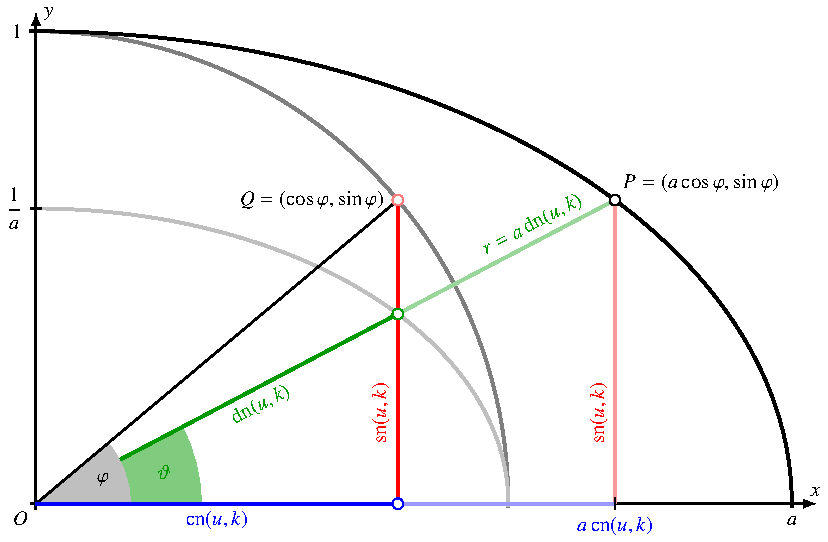
\includegraphics{chapters/110-elliptisch/images/jacobidef.pdf}
\caption{Definition der elliptischen Funktionen als Trigonometrie
an einer Ellipse mit Halbachsen $a$ und $1$.
\label{buch:elliptisch:fig:jacobidef}}
\end{figure}
\subsubsection{Definition der Jacobischen elliptischen Funktionen}
Die elliptischen Funktionen für einen Punkt $P$ auf der Ellipse mit Modulus $k$
können jetzt als Verhältnisse der Koordinaten des Punktes definieren.
Es stellt sich aber die Frage, was man als Argument verwenden soll.
Es soll so etwas wie den Winkel $\varphi$ zwischen der $x$-Achse und dem
Radiusvektor zum Punkt $P$
darstellen, aber wir haben hier noch eine Wahlfreiheit, die wir später
ausnützen möchten.
Im Moment müssen wir die Frage noch nicht beantworten und nennen das
noch unbestimmte Argument $u$.
Wir kümmern uns später um die Frage, wie $u$ von $\varphi$ abhängt.

Die Funktionen, die wir definieren wollen, hängen ausserdem auch 
vom Modulus ab.
Falls der verwendete Modulus aus dem Zusammenhang klar ist, lassen
wir das $k$-Argument weg.

Die Punkte auf dem Einheitskreis haben alle den gleichen Abstand vom
Nullpunkt, dies ist gleichzeitig die definierende Gleichung $r^2=x^2+y^2=1$
des Kreises.
Die Punkte auf der Ellipse erfüllen die Gleichung $x^2/a^2+y^2=1$,
die Entfernung der Punkte $r=\sqrt{x^2+y^2}$ vom Nullpunkt variert aber.

In Analogie zu den trigonometrischen Funktionen setzen wir jetzt für 
die Funktionen
\[
\begin{aligned}
&\text{sinus amplitudinis:}&
{\color{red}\operatorname{sn}(u,k)}&= y \\
&\text{cosinus amplitudinis:}&
{\color{blue}\operatorname{cn}(u,k)}&= \frac{x}{a} \\
&\text{delta amplitudinis:}&
{\color{darkgreen}\operatorname{dn}(u,k)}&=\frac{r}{a},
\end{aligned}
\]
die auch in Abbildung~\ref{buch:elliptisch:fig:jacobidef}
dargestellt sind.
Aus der Gleichung der Ellipse folgt sofort, dass
\[
\operatorname{sn}(u,k)^2 + \operatorname{cn}(u,k)^2 = 1
\]
ist.
Der Satz von Pythagoras kann verwendet werden, um die Entfernung zu
berechnen, also gilt
\begin{equation}
r^2
=
a^2 \operatorname{dn}(u,k)^2
=
x^2 + y^2
=
a^2\operatorname{cn}(u,k)^2 + \operatorname{sn}(u,k)^2
\quad
\Rightarrow
\quad
a^2 \operatorname{dn}(u,k)^2
=
a^2\operatorname{cn}(u,k)^2 + \operatorname{sn}(u,k)^2.
\label{buch:elliptisch:eqn:sncndnrelation}
\end{equation}
Ersetzt man
$
a^2\operatorname{cn}(u,k)^2
=
a^2-a^2\operatorname{sn}(u,k)^2
$, ergibt sich
\[
a^2 \operatorname{dn}(u,k)^2
=
a^2-a^2\operatorname{sn}(u,k)^2
+
\operatorname{sn}(u,k)^2
\quad
\Rightarrow
\quad
\operatorname{dn}(u,k)^2
+
\frac{a^2-1}{a^2}\operatorname{sn}(u,k)^2
=
1,
\]
woraus sich die Identität
\[
\operatorname{dn}(u,k)^2 + k^2 \operatorname{sn}(u,k)^2 = 1
\]
ergibt.
Ebenso kann man aus~\eqref{buch:elliptisch:eqn:sncndnrelation}
die Funktion $\operatorname{cn}(u,k)$ eliminieren, was auf
\[
a^2\operatorname{dn}(u,k)^2
=
a^2\operatorname{cn}(u,k)^2
+1-\operatorname{cn}(u,k)^2
=
(a^2-1)\operatorname{cn}(u,k)^2
+1.
\]
Nach Division durch $a^2$ ergibt sich
\begin{align*}
\operatorname{dn}(u,k)^2
-
k^2\operatorname{cn}(u,k)^2
&=
\frac{1}{a^2}
=
\frac{a^2-a^2+1}{a^2}
=
1-k^2 =: k^{\prime 2}.
\end{align*}
Wir stellen die hiermit gefundenen Relationen zwischen den grundlegenden
Jacobischen elliptischen Funktionen für später zusammen in den Formeln
\begin{equation}
\begin{aligned}
\operatorname{sn}^2(u,k)
+
\operatorname{cn}^2(u,k)
&=
1
\\
\operatorname{dn}^2(u,k) + k^2\operatorname{sn}^2(u,k)
&=
1
\\
\operatorname{dn}^2(u,k)  -k^2\operatorname{cn}^2(u,k)
&=
k^{\prime 2}.
\end{aligned}
\label{buch:elliptisch:eqn:jacobi-relationen}
\end{equation}
zusammen.
So wie es möglich ist, $\sin\alpha$ durch $\cos\alpha$ auszudrücken,
ist es mit
\eqref{buch:elliptisch:eqn:jacobi-relationen}
jetzt auch möglich jede grundlegende elliptische Funktion durch
jede anderen auszudrücken.
Die Resultate sind in der Tabelle~\ref{buch:elliptisch:fig:jacobi-relationen}
zusammengestellt.

\begin{table}
\centering
\renewcommand{\arraystretch}{2.1}
\begin{tabular}{|>{$\displaystyle}c<{$}|>{$\displaystyle}c<{$}>{$\displaystyle}c<{$}>{$\displaystyle}c<{$}|}
\hline
&\operatorname{sn}(u,k)
&\operatorname{cn}(u,k)
&\operatorname{dn}(u,k)\\
\hline
\operatorname{sn}(u,k)
&\operatorname{sn}(u,k)
&\sqrt{1-\operatorname{cn}^2(u,k)}
&\frac1k\sqrt{1-\operatorname{dn}^2(u,k)}
\\
\operatorname{cn}(u,k)
&\sqrt{1-\operatorname{sn}^2(u,k)}
&\operatorname{cn}(u,k)
&\frac{1}{k}\sqrt{\operatorname{dn}^2(u,k)-k^{\prime2}}
\\
\operatorname{dn}(u,k)
&\sqrt{1-k^2\operatorname{sn}^2(u,k)}
&\sqrt{k^{\prime2}+k^2\operatorname{cn}^2(u,k)}
&\operatorname{dn}(u,k)
\\
\hline
\end{tabular}
\caption{Jede der Jacobischen elliptischen Funktionen lässt sich
unter Verwendung der Relationen~\eqref{buch:elliptisch:eqn:jacobi-relationen}
durch jede andere ausdrücken.
\label{buch:elliptisch:fig:jacobi-relationen}}
\end{table}

%
% Ableitungen der Jacobi-ellpitischen Funktionen
% 
\subsubsection{Ableitung}
Die trigonometrischen Funktionen sind deshalb so besonders nützlich 
für die Lösung von Schwingungsdifferentialgleichungen, weil sie die
Beziehungen
\[
\frac{d}{d\varphi}  \cos\varphi = -\sin\varphi
\qquad\text{und}\qquad
\frac{d}{d\varphi}  \sin\varphi = \cos\varphi
\]
erfüllen.
So einfach können die Beziehungen natürlich nicht sein, sonst würde sich
durch Integration ja wieder nur die trigonometrischen Funktionen ergeben.
Durch geschickte Wahl des Arguments $u$ kann man aber erreichen, dass
sie ähnlich nützliche Beziehungen zwischen den Ableitungen ergeben.

Gesucht ist jetzt also eine Wahl für das Argument $u$ zum Beispiel in
Abhängigkeit von $\varphi$, dass sich einfache und nützliche
Ableitungsformeln ergeben.
Wir setzen daher $u(\varphi)$ voraus und beachten, dass $x$ und $y$
ebenfalls von $\varphi$ abhängen, es ist
$y=\sin\varphi$ und $x=a\cos\varphi$.
Die Ableitungen von $x$ und $y$ nach $\varphi$ sind
\begin{align*}
\frac{dy}{d\varphi}
&=
\cos\varphi
=
\frac{1}{a} x
=
\operatorname{cn}(u,k)
\\
\frac{dx}{d\varphi}
&=
-a\sin\varphi
=
-a y
=
-a\operatorname{sn}(u,k).
\end{align*}
Daraus kann man jetzt die folgenden Ausdrücke für die Ableitungen der
elliptischen Funktionen nach $\varphi$ ableiten:
\begin{align*}
\frac{d}{d\varphi} \operatorname{sn}(u,z)
&=
\frac{d}{d\varphi} y(\varphi)
=
\cos\varphi
=
\frac{x}{a}
=
\operatorname{cn}(u,k)
&&\Rightarrow&
\frac{d}{du}
\operatorname{sn}(u,k)
&=
\operatorname{cn}(u,k) \frac{d\varphi}{du}
\\
\frac{d}{d\varphi} \operatorname{cn}(u,z)
&=
\frac{d}{d\varphi} \frac{x(\varphi)}{a}
=
-\sin\varphi
=
-\operatorname{sn}(u,k)
&&\Rightarrow&
\frac{d}{du}\operatorname{cn}(u,k)
&=
-\operatorname{sn}(u,k) \frac{d\varphi}{du}
\\
\frac{d}{d\varphi} \operatorname{dn}(u,z)
&=
\frac{1}{a}\frac{dr}{d\varphi}
=
\frac{1}{a}\frac{d\sqrt{x^2+y^2}}{d\varphi}
%\\
%&
\rlap{$\displaystyle\mathstrut
=
\frac{x}{ar} \frac{dx}{d\varphi}
+
\frac{y}{ar} \frac{dy}{d\varphi}
%\\
%&
=
\frac{x}{ar} (-a\operatorname{sn}(u,k))
+
\frac{y}{ar} \operatorname{cn}(u,k)
$}
\\
&
\rlap{$\displaystyle\mathstrut
=
\frac{x}{ar}(-ay)
+
\frac{y}{ar} \frac{x}{a}
%\rlap{$\displaystyle
=
\frac{xy(-1+\frac{1}{a^2})}{r} 
%$}
%\\
%&
=
-\frac{xy(a^2-1)}{a^2r} 
$}
\\
&=
-\frac{a^2-1}{ar}
\operatorname{cn}(u,k) \operatorname{sn}(u,k)
%\\
%&
\rlap{$\displaystyle\mathstrut
=
-k^2
\frac{a}{r}
\operatorname{cn}(u,k) \operatorname{sn}(u,k)
$}
\\
&=
-k^2\frac{\operatorname{cn}(u,k)\operatorname{sn}(u,k)}{\operatorname{dn}(u,k)}
&&\Rightarrow&
\frac{d}{du} \operatorname{dn}(u,k)
&=
-k^2\frac{\operatorname{cn}(u,k)
\operatorname{sn}(u,k)}{\operatorname{dn}(u,k)}
\frac{d\varphi}{du}.
\end{align*}
Die einfachsten Beziehungen ergeben sich offenbar, wenn man $u$ so
wählt, dass
\[
\frac{d\varphi}{du}
=
\operatorname{dn}(u,k)
=
\frac{r}{a}.
\]
Damit haben wir die im folgenden Satz zusammengefassten
grundlegenden Ableitungsregeln der Jacobischen elliptischen Funktionen
gefunden.

\begin{satz}
\index{Satz!Ableitungen der Jacobischen elliptischen Funktionen}%
\label{buch:elliptisch:satz:ableitungen}
Die Jacobischen elliptischen Funktionen haben die Ableitungen
\begin{equation}
\begin{aligned}
\frac{d}{du}\operatorname{sn}(u,k)
&=
\phantom{-}\operatorname{cn}(u,k)\operatorname{dn}(u,k)
\\
\frac{d}{du}\operatorname{cn}(u,k)
&=
-\operatorname{sn}(u,k)\operatorname{dn}(u,k)
\\
\frac{d}{du}\operatorname{dn}(u,k)
&=
-k^2\operatorname{sn}(u,k)\operatorname{cn}(u,k).
\end{aligned}
\label{buch:elliptisch:eqn:ableitungsregeln}
\end{equation}
\end{satz}

%
% Der Grenzfall $k=1$
%
\subsubsection{Der Grenzwert $k\to1$}
\begin{figure}
\centering
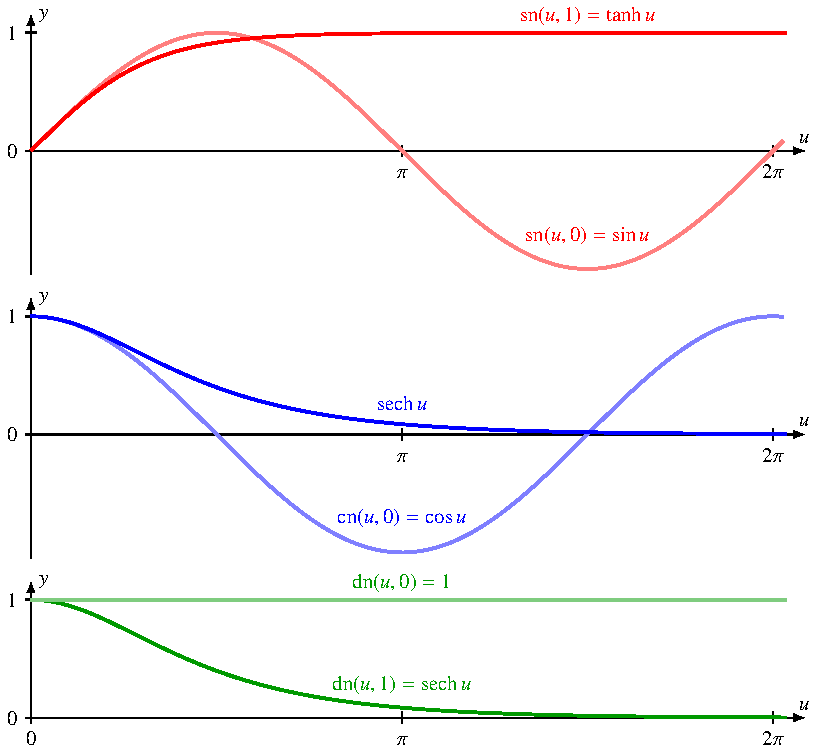
\includegraphics{chapters/110-elliptisch/images/sncnlimit.pdf}
\caption{Grenzfälle der Jacobischen elliptischen Funktionen 
für die Werte $0$ und $1$ des Parameters $k$.
\label{buch:elliptisch:fig:sncnlimit}}
\end{figure}
Für $k=1$ ist $k^{\prime2}=1-k^2=$ und es folgt aus den
Relationen~\eqref{buch:elliptisch:eqn:jacobi-relationen}
\[
\operatorname{cn}^2(u,k)
-
k^2
\operatorname{dn}^2(u,k)
=
k^{\prime2}
=
0
\qquad\Rightarrow\qquad
\operatorname{cn}^2(u,1)
=
\operatorname{dn}^2(u,1),
\]
die beiden Funktionen
$\operatorname{cn}(u,k)$
und
$\operatorname{dn}(u,k)$
fallen also zusammen.
Die Ableitungsregeln werden dadurch vereinfacht:
\begin{align*}
\operatorname{sn}'(u,1)
&=
\operatorname{cn}(u,1)
\operatorname{dn}(u,1)
=
\operatorname{cn}^2(u,1)
=
1-\operatorname{sn}^2(u,1)
&&\Rightarrow& y'&=1-y^2
\\
\operatorname{cn}'(u,1)
&=
-
\operatorname{sn}(u,1)
\operatorname{dn}(u,1)
=
-
\operatorname{sn}(u,1)\operatorname{cn}(u,1)
&&\Rightarrow&
\frac{z'}{z}&=(\log z)' = -y.
\end{align*}
Die erste Differentialgleichung für $y$ lässt sich separieren, man findet
die Lösung
\[
\frac{y'}{1-y^2}
=
1
\quad\Rightarrow\quad
\int \frac{dy}{1-y^2} = \int \,du
\quad\Rightarrow\quad
\operatorname{artanh}(y) = u
\quad\Rightarrow\quad
\operatorname{sn}(u,1)=\tanh u.
\]
Damit kann man jetzt auch $z$ berechnen:
\begin{align*}
(\log \operatorname{cn}(u,1))'
&=
\tanh u
&&\Rightarrow&
\log\operatorname{cn}(u,1)
&=
-\int\tanh u\,du
=
-\log\cosh u
\\
&
&&\Rightarrow&
\operatorname{cn}(u,1)
&=
\frac{1}{\cosh u}
=
\operatorname{sech}u.
\end{align*}
Die Grenzfunktionen sind in Abbildung~\ref{buch:elliptisch:fig:sncnlimit}
dargestellt.

%
% Das Argument u
%
\subsubsection{Das Argument $u$}
Die Gleichung 
\begin{equation}
\frac{d\varphi}{du}
=
\operatorname{dn}(u,k)
\label{buch:elliptisch:eqn:uableitung}
\end{equation}
ermöglicht, $\varphi$ in Abhängigkeit von $u$ zu berechnen, ohne jedoch
die geometrische Bedeutung zu klären.
Das beginnt bereits damit, dass der Winkel $\varphi$ nicht nicht der
Polarwinkel des Punktes $P$ in Abbildung~\ref{buch:elliptisch:fig:jacobidef}
ist, diesen nennen wir $\vartheta$.
Der Zusammenhang zwischen $\varphi$ und $\vartheta$ ist
\begin{equation}
\frac1{a}\tan\varphi = \tan\vartheta.
\label{buch:elliptisch:eqn:phitheta}
\end{equation}

Um die geometrische Bedeutung besser zu verstehen, nehmen wir jetzt an,
dass die Ellipse mit einem Parameter $t$ parametrisiert ist, dass also
$\varphi(t)$, $\vartheta(t)$ und $u(t)$ Funktionen von $t$ sind.
Die Ableitung von~\eqref{buch:elliptisch:eqn:phitheta} ist
\[
\frac1{a}\cdot \frac{1}{\cos^2\varphi}\cdot \dot{\varphi}
=
\frac{1}{\cos^2\vartheta}\cdot \dot{\vartheta}.
\]
Daraus kann die Ableitung von $\vartheta$ nach $\varphi$ bestimmt
werden, sie ist
\[
\frac{d\vartheta}{d\varphi}
=
\frac{\dot{\vartheta}}{\dot{\varphi}}
=
\frac{1}{a}
\cdot
\frac{\cos^2\vartheta}{\cos^2\varphi}
=
\frac{1}{a}
\cdot
\frac{(x/r)^2}{(x/a)^2}
=
\frac{1}{a}\cdot
\frac{a^2}{r^2}
=
\frac{1}{a}\cdot\frac{1}{\operatorname{dn}^2(u,k)}.
\]
Damit kann man jetzt mit Hilfe von~\eqref{buch:elliptisch:eqn:uableitung} 
Die Ableitung von $\vartheta$ nach $u$ ermitteln, sie ist
\[
\frac{d\vartheta}{du}
=
\frac{d\vartheta}{d\varphi}
\cdot
\frac{d\varphi}{du}
=
\frac{1}{a}\cdot\frac{1}{\operatorname{dn}^2(u,k)}
\cdot
\operatorname{dn}(u,k)
=
\frac{1}{a}
\cdot
\frac{1}{\operatorname{dn}(u,k)}
=
\frac{1}{a}
\cdot\frac{a}{r}
=
\frac{1}{r},
\]
wobei wir auch die Definition der Funktion $\operatorname{dn}(u,k)$
verwendet haben.

In der Parametrisierung mit dem Parameter $t$ kann man jetzt die Ableitung
von $u$ nach $t$ berechnen als
\[
\frac{du}{dt}
=
\frac{du}{d\vartheta}
\frac{d\vartheta}{dt}
=
r
\dot{\vartheta}.
\]
Darin ist $\dot{\vartheta}$ die Winkelgeschwindigkeit des Punktes um
das Zentrum $O$ und $r$ ist die aktuelle Entfernung des Punktes $P$
von $O$.
$r\dot{\vartheta}$ ist also die Geschwindigkeitskomponenten des Punktes
$P$ senkrecht auf den aktuellen Radiusvektor.
Der Parameter $u$, der zum Punkt $P$ gehört, ist also das Integral
\[
u(P) = \int_0^P r\,d\vartheta.
\]
Für einen Kreis ist die Geschwindigkeit von $P$ immer senkrecht
auf dem Radiusvektor und der Radius ist konstant, so dass
$u(P)=\vartheta(P)$ ist.

%
% Die abgeleiteten elliptischen Funktionen
%
\begin{figure}
\centering
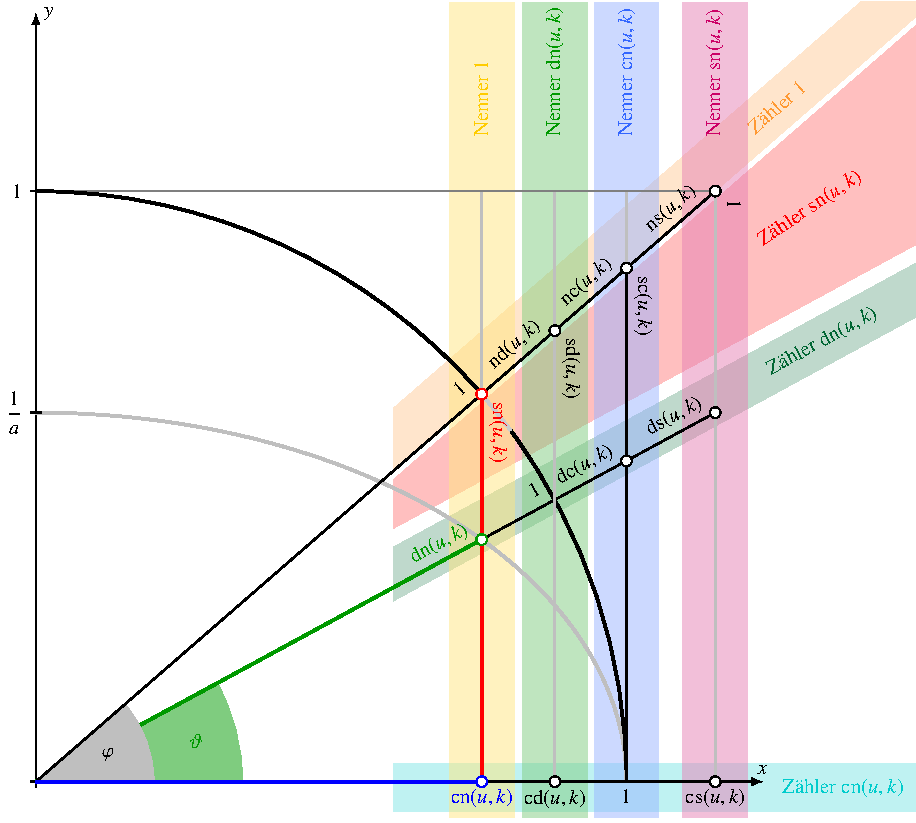
\includegraphics[width=\textwidth]{chapters/110-elliptisch/images/jacobi12.pdf}
\caption{Die Verhältnisse der Funktionen
$\operatorname{sn}(u,k)$,
$\operatorname{cn}(u,k)$
udn
$\operatorname{dn}(u,k)$
geben Anlass zu neun weitere Funktionen, die sich mit Hilfe
des Strahlensatzes geometrisch interpretieren lassen.
\label{buch:elliptisch:fig:jacobi12}}
\end{figure}
\begin{table}
\centering
\renewcommand{\arraystretch}{2.5}
\begin{tabular}{|>{$\displaystyle}c<{$}|>{$\displaystyle}c<{$}>{$\displaystyle}c<{$}>{$\displaystyle}c<{$}>{$\displaystyle}c<{$}|}
\hline
\cdot &
\frac{1}{1} &
\frac{1}{\operatorname{sn}(u,k)} &
\frac{1}{\operatorname{cn}(u,k)} &
\frac{1}{\operatorname{dn}(u,k)} 
\\[5pt]
\hline
1&
&%\operatorname{nn}(u,k)=\frac{1}{1} &
\operatorname{ns}(u,k)=\frac{1}{\operatorname{sn}(u,k)} &
\operatorname{nc}(u,k)=\frac{1}{\operatorname{cn}(u,k)} &
\operatorname{nd}(u,k)=\frac{1}{\operatorname{dn}(u,k)}
\\
\operatorname{sn}(u,k) &
\operatorname{sn}(u,k)=\frac{\operatorname{sn}(u,k)}{1}&
&%\operatorname{ss}(u,k)=\frac{\operatorname{sn}(u,k)}{\operatorname{sn}(u,k)}&
\operatorname{sc}(u,k)=\frac{\operatorname{sn}(u,k)}{\operatorname{cn}(u,k)}&
\operatorname{sd}(u,k)=\frac{\operatorname{sn}(u,k)}{\operatorname{dn}(u,k)}
\\
\operatorname{cn}(u,k) &
\operatorname{cn}(u,k)=\frac{\operatorname{cn}(u,k)}{1} &
\operatorname{cs}(u,k)=\frac{\operatorname{cn}(u,k)}{\operatorname{sn}(u,k)}&
&%\operatorname{cc}(u,k)=\frac{\operatorname{cn}(u,k)}{\operatorname{cn}(u,k)}&
\operatorname{cd}(u,k)=\frac{\operatorname{cn}(u,k)}{\operatorname{dn}(u,k)}
\\
\operatorname{dn}(u,k) &
\operatorname{dn}(u,k)=\frac{\operatorname{dn}(u,k)}{1} &
\operatorname{ds}(u,k)=\frac{\operatorname{dn}(u,k)}{\operatorname{sn}(u,k)}&
\operatorname{dc}(u,k)=\frac{\operatorname{dn}(u,k)}{\operatorname{cn}(u,k)}&
%\operatorname{dd}(u,k)=\frac{\operatorname{dn}(u,k)}{\operatorname{dn}(u,k)}
\\[5pt]
\hline
\end{tabular}
\caption{Zusammenstellung der abgeleiteten Jacobischen elliptischen
Funktionen in hinteren drei Spalten als Quotienten der grundlegenden
Jacobischen elliptischen Funktionen.
Die erste Spalte zum Nenner $1$ enthält die grundlegenden
Jacobischen elliptischen Funktionen.
\label{buch:elliptisch:table:abgeleitetjacobi}}
\end{table}

%
% Die abgeleiteten elliptischen Funktionen
%
\subsubsection{Die abgeleiteten elliptischen Funktionen}
Zusätzlich zu den grundlegenden Jacobischen elliptischen Funktioenn
lassen sich weitere elliptische Funktionen bilden, die unglücklicherweise
die {\em abgeleiteten elliptischen Funktionen} genannt werden.
Ähnlich wie die trigonometrischen Funktionen $\tan\alpha$, $\cot\alpha$,
$\sec\alpha$ und $\csc\alpha$ als Quotienten von $\sin\alpha$ und
$\cos\alpha$ definiert sind, sind die abgeleiteten elliptischen Funktionen
die in Tabelle~\ref{buch:elliptisch:table:abgeleitetjacobi} zusammengestellten
Quotienten der grundlegenden Jacobischen elliptischen Funktionen.
Die Bezeichnungskonvention ist, dass die Funktion $\operatorname{pq}(u,k)$
ein Quotient ist, dessen Zähler durch den Buchstaben p bestimmt ist,
der Nenner durch den Buchstaben q.
Der Buchstabe n steht für eine $1$, die Buchstaben s, c und d stehen für
die Anfangsbuchstaben der grundlegenden Jacobischen elliptischen
Funktionen.
Meint man irgend eine der Jacobischen elliptischen Funktionen, schreibt
man manchmal auch $\operatorname{zn}(u,k)$.

In Abbildung~\ref{buch:elliptisch:fig:jacobi12} sind die Quotienten auch
geometrisch interpretiert.
Der Wert der Funktion $\operatorname{nq}(u,k)$ ist die auf dem Strahl
mit Polarwinkel $\varphi$ abgetragene Länge bis zu den vertikalen
Geraden, die den verschiedenen möglichen Nennern entsprechen.
Entsprechend ist der Wert der Funktion $\operatorname{dq}(u,k)$ die
Länge auf dem Strahl mit Polarwinkel $\vartheta$.

Die Relationen~\ref{buch:elliptisch:eqn:jacobi-relationen}
ermöglichen, jede Funktion $\operatorname{zn}(u,k)$ durch jede
andere auszudrücken.
Die schiere Anzahl solcher Beziehungen macht es unmöglich, sie 
übersichtlich in einer Tabelle zusammenzustellen, daher soll hier
nur an einem Beispiel das Vorgehen gezeigt werden:

\begin{beispiel}
Die Funktion $\operatorname{sc}(u,k)$ soll durch $\operatorname{cd}(u,k)$
ausgedrückt werden.
Zunächst ist 
\[
\operatorname{sc}(u,k)
=
\frac{\operatorname{sn}(u,k)}{\operatorname{cn}(u,k)}
\]
nach Definition.
Im Resultat sollen nur noch $\operatorname{cn}(u,k)$ und
$\operatorname{dn}(u,k)$ vorkommen.
Daher eliminieren wir zunächst die Funktion $\operatorname{sn}(u,k)$
mit Hilfe von \eqref{buch:elliptisch:eqn:jacobi-relationen} und erhalten
\begin{equation}
\operatorname{sc}(u,k)
=
\frac{\sqrt{1-\operatorname{cn}^2(u,k)}}{\operatorname{cn}(u,k)}.
\label{buch:elliptisch:eqn:allgausdruecken}
\end{equation}
Nun genügt es, die Funktion $\operatorname{cn}(u,k)$ durch
$\operatorname{cd}(u,k)$ auszudrücken.
Aus der Definition und der
dritten Relation in \eqref{buch:elliptisch:eqn:jacobi-relationen} 
erhält man
\begin{align*}
\operatorname{cd}^2(u,k)
&=
\frac{\operatorname{cn}^2(u,k)}{\operatorname{dn}^2(u,k)}
=
\frac{\operatorname{cn}^2(u,k)}{k^{\prime2}+k^2\operatorname{cn}^2(u,k)}
\\
\Rightarrow
\qquad
k^{\prime 2}
\operatorname{cd}^2(u,k)
+
k^2\operatorname{cd}^2(u,k)\operatorname{cn}^2(u,k)
&=
\operatorname{cn}^2(u,k)
\\
\operatorname{cn}^2(u,k)
-
k^2\operatorname{cd}^2(u,k)\operatorname{cn}^2(u,k)
&=
k^{\prime 2}
\operatorname{cd}^2(u,k)
\\
\operatorname{cn}^2(u,k)
&=
\frac{
k^{\prime 2}
\operatorname{cd}^2(u,k)
}{
1 - k^2\operatorname{cd}^2(u,k)
}.
\end{align*}
Für den Zähler brauchen wir $1-\operatorname{cn}^2(u,k)$, also
\[
1-\operatorname{cn}^2(u,k)
=
\frac{
1
-
k^2\operatorname{cd}^2(u,k)
-
k^{\prime 2}
\operatorname{cd}^2(u,k)
}{
1
-
k^2\operatorname{cd}^2(u,k)
}
=
\frac{1-\operatorname{cd}^2(u,k)}{1-k^2\operatorname{cd}^2(u,k)}.
\]
Einsetzen in~\eqref{buch:elliptisch:eqn:allgausdruecken} gibt
\begin{align*}
\operatorname{sc}(u,k)
&=
\frac{
\sqrt{1-\operatorname{cd}^2(u,k)}
}{\sqrt{1-k^2\operatorname{cd}^2(u,k)}}
\cdot
\frac{
\sqrt{1 - k^2\operatorname{cd}^2(u,k)}
}{
k'
\operatorname{cd}(u,k)
}
=
\frac{
\sqrt{1-\operatorname{cd}^2(u,k)}
}{
k'
\operatorname{cd}(u,k)
}.
\qedhere
\end{align*}
\end{beispiel}

\subsubsection{Ableitung der abgeleiteten elliptischen Funktionen}
Aus den Ableitungen der grundlegenden Jacobischen elliptischen Funktionen
können mit der Quotientenregel nun auch beliebige Ableitungen der
abgeleiteten Jacobischen elliptischen Funktionen gefunden werden.
Als Beispiel berechnen wir die Ableitung von $\operatorname{sc}(u,k)$.
Sie ist
\begin{align*}
\frac{d}{du}
\operatorname{sc}(u,k)
&=
\frac{d}{du}
\frac{\operatorname{sn}(u,k)}{\operatorname{cn}(u,k)}
=
\frac{
\operatorname{sn}'(u,k)\operatorname{cn}(u,k)
-
\operatorname{sn}(u,k)\operatorname{cn}'(u,k)}{
\operatorname{cn}^2(u,k)
}
\\
&=
\frac{
\operatorname{cn}^2(u,k)\operatorname{dn}(u,k)
+
\operatorname{sn}^2(u,k)\operatorname{dn}(u,k)
}{
\operatorname{cn}^2(u,k)
}
=
\frac{(
\operatorname{sn}^2(u,k)
+
\operatorname{cn}^2(u,k)
)\operatorname{dn}(u,k)}{
\operatorname{cn}^2(u,k)
}
\\
&=
\frac{1}{\operatorname{cn}(u,k)}
\cdot
\frac{\operatorname{dn}(u,k)}{\operatorname{cn}(u,k)}
=
\operatorname{nc}(u,k)
\operatorname{dc}(u,k).
\end{align*}
Man beachte, dass das Quadrat der Nennerfunktion im Resultat
der Quotientenregel zur Folge hat, dass die
beiden Funktionen im Resultat beide den gleichen Nenner haben wie
die Funktion, die abgeleitet wird.

Mit etwas Fleiss kann man nach diesem Muster alle Ableitungen
\begin{equation}
%\small
\begin{aligned}
\operatorname{sn}'(u,k)
&= 
\phantom{-}
\operatorname{cn}(u,k)\,\operatorname{dn}(u,k)
&&\qquad&
\operatorname{ns}'(u,k)
&=
-
\operatorname{cs}(u,k)\,\operatorname{ds}(u,k)
\\
\operatorname{cn}'(u,k)
&= 
-
\operatorname{sn}(u,k)\,\operatorname{dn}(u,k)
&&&
\operatorname{nc}'(u,k)
&=
\phantom{-}
\operatorname{sc}(u,k)\,\operatorname{dc}(u,k)
\\
\operatorname{dn}'(u,k)
&= 
-k^2
\operatorname{sn}(u,k)\,\operatorname{cn}(u,k)
&&&
\operatorname{nd}'(u,k)
&=
\phantom{-}
k^2
\operatorname{sd}(u,k)\,\operatorname{cd}(u,k)
\\
\operatorname{sc}'(u,k)
&=
\phantom{-}
\operatorname{dc}(u,k)\,\operatorname{nc}(u,k)
&&&
\operatorname{cs}'(u,k)
&=
-
\operatorname{ds}(u,k)\,\operatorname{ns}(u,k)
\\
\operatorname{cd}'(u,k)
&=
-k^{\prime2}
\operatorname{sd}(u,k)\,\operatorname{nd}(u,k)
&&&
\operatorname{dc}'(u,k)
&=
\phantom{-}
k^{\prime2}
\operatorname{dc}(u,k)\,\operatorname{nc}(u,k)
\\
\operatorname{ds}'(d,k)
&=
-
\operatorname{cs}(u,k)\,\operatorname{ns}(u,k)
&&&
\operatorname{sd}'(d,k)
&=
\phantom{-}
\operatorname{cd}(u,k)\,\operatorname{nd}(u,k)
\end{aligned}
\label{buch:elliptisch:eqn:alleableitungen}
\end{equation}
finden.
Man beachte, dass in jeder Identität alle Funktionen den gleichen
zweiten Buchstaben haben.

\subsubsection{Weitere Beziehungen}
Für die Jacobischen elliptischen Funktionen lässt sich eine grosse
Zahl weiterer Eigenschaften und Identitäten beweisen.
Zum Beispiel gibt es Aditionstheoreme, die im Grenzfall $k\to 0$ zu
den Additionstheoremen für die trigonometrischen Funktionen werden.
\index{Additionstheorem}%
Ebenso kann man weitere algebraische Identitäten finden.
So lässt sich zum Beispiel die einzige reelle Nullstelle von $x^5+x=w$
mit Jacobischen elliptischen Funktionen darstellen, während es
nicht möglich ist, diese Lösung als Wurzelausdruck zu schreiben.

Die Jacobischen elliptischen Funktionen lassen sich statt auf dem
hier gewählten trigonometrischen Weg auch mit Hilfe der Jacobischen
Theta-Funktionen definieren, die Lösungen einer Wärmeleitungsgleichung
\index{Theta-Funktionen}%
\index{Wärmeleitungs-Gleichung}%
mit geeigneten Randbedingungen sind.
Diese Vorgehensweise hat den Vorteil, ziemlich direkt zu
Reihen- und Produktentwicklungen für die Funktionen zu führen.
Auch die Additionstheorem ergeben sich vergleichsweise leicht.
Dieser Zugang zu den Jacobischen elliptischen Funktionen wird in der
Standardreferenz~\cite{buch:ellfun-applications} gewählt.

Bei anderen speziellen Funktionen waren Reihenentwicklungen ein
wichtiges Hilfsmittel zu deren numerischer Berechnung.
Bei den Jacobischen elliptischen Funktionen ist diese Methode
nicht zielführend.
Im Abschnitt~\ref{buch:elliptisch:subsection:differentialgleichungen}
wird gezeigt, dass Jacobische elliptische Funktionen gewisse nichtlineare
Differentialgleichungen zu lösen ermöglichen.
Dies zeigt auch, dass Jacobischen elliptischen Funktionen
Umkehrfunktionen der elliptischen Integrale sind, die in
Abschnitt~\ref{buch:elliptisch:subsection:agm} mit dem
arithmetisch-geometrischen Mittel berechnet wurden.
Die dort angetroffenen numerischen Schwierigkeiten treten bei der
Berechnung der Umkehrfunktion jedoch nicht auf.

Die grundlegende Mechanik dieser Berechnungsmethode wird auf
Seite~\pageref{buch:elliptisch:jacobi:agm} dargestellt und
und in den Übungsaufgaben
\ref{buch:elliptisch:aufgabe:2} bis \ref{buch:elliptisch:aufgabe:5}
etwas näher untersucht wird.

Aus der Theorie das arithmetisch-geometrischen Mittels lässt sich
die sogenannte Landen-Trans\-formation herleiten.
\index{Landen-Transformation}%
Sie stellt eine Verbindung zwischen
den Werten der elliptischen Funktionen zu verschiedenen Moduli $k$ her.
Sie ist die Basis aller effizienten Berechnungsmethoden.


% algebraische Beziehungen \\
% Additionstheoreme \\
% Perioden
% use https://math.stackexchange.com/questions/3013692/how-to-show-that-jacobi-sine-function-is-doubly-periodic



%
% 22-dglsol.tex -- Lösung von Differentialgleichungen
%
% (c) 2021 Prof Dr Andreas Müller, OST Ostschweizer Fachhochschule
%

%
% Lösung von Differentialgleichungen
%
\subsection{Lösungen von Differentialgleichungen
\label{buch:elliptisch:subsection:differentialgleichungen}}
Die elliptischen Funktionen ermöglichen die Lösung gewisser nichtlinearer
Differentialgleichungen in geschlossener Form.
Ziel dieses Abschnitts ist, Differentialgleichungen der Form
\(
\dot{x}(t)^2
=
P(x(t))
\)
mit einem Polynom $P$ vierten Grades oder
\(
\ddot{x}(t)
=
p(x(t))
\)
mit einem Polynom dritten Grades als rechter Seite lösen zu können.

%
% Die Differentialgleichung der elliptischen Funktionen
%
\subsubsection{Die Differentialgleichungen der elliptischen Funktionen}
Um Differentialgleichungen mit elliptischen Funktion lösen zu
können, muss man als erstes die Differentialgleichungen derselben
finden.
Quadriert man die Ableitungsregel für $\operatorname{sn}(u,k)$, erhält
man
\[
\biggl(\frac{d}{du}\operatorname{sn}(u,k)\biggr)^2
=
\operatorname{cn}(u,k)^2 \operatorname{dn}(u,k)^2.
\]
Die Funktionen auf der rechten Seite können durch $\operatorname{sn}(u,k)$
ausgedrückt werden, dies führt auf die Differentialgleichung
\begin{align*}
\biggl(\frac{d}{du}\operatorname{sn}(u,k)\biggr)^2
&=
\bigl(
1-\operatorname{sn}(u,k)^2
\bigr)
\bigl(
1-k^2 \operatorname{sn}(u,k)^2
\bigr)
\\
&=
k^2\operatorname{sn}(u,k)^4 
-(1+k^2)
\operatorname{sn}(u,k)^2 
+1.
\end{align*}
Für die Funktion $\operatorname{cn}(u,k)$ ergibt die analoge Rechnung
\begin{align*}
\frac{d}{du}\operatorname{cn}(u,k)
&=
-\operatorname{sn}(u,k) \operatorname{dn}(u,k)
\\
\biggl(\frac{d}{du}\operatorname{cn}(u,k)\biggr)^2
&=
\operatorname{sn}(u,k)^2 \operatorname{dn}(u,k)^2
\\
&=
\bigl(1-\operatorname{cn}(u,k)^2\bigr)
\bigl(k^{\prime 2}+k^2 \operatorname{cn}(u,k)^2\bigr)
\\
&=
-k^2\operatorname{cn}(u,k)^4
+
(k^2-k^{\prime 2})\operatorname{cn}(u,k)^2
+
k^{\prime 2}
\intertext{und weiter für $\operatorname{dn}(u,k)$:}
\frac{d}{du}\operatorname{dn}(u,k)
&=
-k^2\operatorname{sn}(u,k)\operatorname{cn}(u,k)
\\
\biggl(
\frac{d}{du}\operatorname{dn}(u,k)
\biggr)^2
&=
\bigl(k^2 \operatorname{sn}(u,k)^2\bigr)
\bigl(k^2 \operatorname{cn}(u,k)^2\bigr)
\\
&=
\bigl(
1-\operatorname{dn}(u,k)^2
\bigr)
\bigl(
\operatorname{dn}(u,k)^2-k^{\prime 2}
\bigr)
\\
&=
-\operatorname{dn}(u,k)^4
+
(1+k^{\prime 2})\operatorname{dn}(u,k)^2
-k^{\prime 2}.
\end{align*}

\begin{table}
\centering
\renewcommand{\arraystretch}{1.7}
\begin{tabular}{|>{$}l<{$}|>{$}l<{$}|>{$}c<{$}|>{$}c<{$}|>{$}c<{$}|}
\hline
\text{Funktion $y=$}&\text{Differentialgleichung}&\alpha&\beta&\gamma\\
\hline
\operatorname{sn}(u,k)
	& y'^2 = \phantom{-}(1-y^2)(1-k^2y^2)
		&k^2&1+k^2&1
\\
\operatorname{cn}(u,k) &y'^2 = \phantom{-}(1-y^2)(k^{\prime2}+k^2y^2)
		&-k^2	&k^2-k^{\prime 2}=2k^2-1&k^{\prime2}
\\
\operatorname{dn}(u,k)
	& y'^2 = -(1-y^2)(k^{\prime 2}-y^2)
		&-1	&1+k^{\prime 2}=2-k^2	&-k^{\prime2}
\\
\hline
\end{tabular}
\caption{Elliptische Funktionen als Lösungsfunktionen für verschiedene
nichtlineare Differentialgleichungen der Art
\eqref{buch:elliptisch:eqn:1storderdglell}.
Die Vorzeichen der Koeffizienten $\alpha$, $\beta$ und $\gamma$
entscheidet darüber, welche Funktion für die Lösung verwendet werden
muss.
\label{buch:elliptisch:tabelle:loesungsfunktionen}}
\end{table}

Die drei grundlegenden Jacobischen elliptischen Funktionen genügen also alle
einer nichtlinearen Differentialgleichung erster Ordnung der selben Art.
Das Quadrat der Ableitung ist ein Polynom vierten Grades der Funktion.
Die Differentialgleichungen sind in der
Tabelle~\ref{buch:elliptisch:tabelle:loesungsfunktionen} zusammengefasst.

%
% Differentialgleichung der abgeleiteten elliptischen Funktionen
%
\subsubsection{Die Differentialgleichung der abgeleiteten elliptischen
Funktionen}
Da auch die Ableitungen der abgeleiteten Jacobischen elliptischen
Funktionen Produkte von genau zwei Funktionen sind, die sich wieder
durch die ursprüngliche Funktion ausdrücken lassen, darf man erwarten,
dass alle elliptischen Funktionen einer ähnlichen Differentialgleichung
genügen.
Um dies besser einzufangen, schreiben wir $\operatorname{pq}(u,k)$,
wenn wir eine beliebige abgeleitete Jacobische elliptische Funktion
meinen.
Für 
$\operatorname{pq}=\operatorname{sn}$,
$\operatorname{pq}=\operatorname{cn}$
und
$\operatorname{pq}=\operatorname{dn}$
wissen wir bereits und erwarten für jede andere Funktion dass
$\operatorname{pq}(u,k)$ auch, dass sie Lösung einer Differentialgleichung
der Form
\begin{equation}
\operatorname{pq}'(u,k)^2
=
\alpha \operatorname{pq}(u,k)^4 + \beta \operatorname{pq}(u,k)^2 + \gamma
\label{buch:elliptisch:eqn:1storderdglell}
\end{equation}
ist,
wobei wir mit $\operatorname{pq}'(u,k)$ die Ableitung von
$\operatorname{pq}(u,k)$ nach dem ersten Argument meinen.
Die Koeffizienten $\alpha$, $\beta$ und $\gamma$ hängen von $k$ ab,
ihre Werte für die grundlegenden Jacobischen elliptischen
sind in Tabelle~\ref{buch:elliptisch:table:differentialgleichungen}
zusammengestellt.

Die Koeffizienten müssen nicht für jede Funktion wieder neu bestimmt
werden, denn für den Kehrwert einer Funktion lässt sich die
Differentialgleichung aus der Differentialgleichung der ursprünglichen
Funktion ermitteln.

%
% Differentialgleichung der Kehrwertfunktion
%
\subsubsection{Differentialgleichung für den Kehrwert einer elliptischen Funktion}
Aus der Differentialgleichung~\eqref{buch:elliptisch:eqn:1storderdglell}
für die Funktion $\operatorname{pq}(u,k)$ kann auch eine
Differentialgleichung für den Kehrwert
$\operatorname{qp}(u,k)=\operatorname{pq}(u,k)^{-1}$
ableiten.
Dazu rechnet man
\[
\operatorname{qp}'(u,k)
=
\frac{d}{du}\frac{1}{\operatorname{pq}(u,k)}
=
\frac{\operatorname{pq}'(u,k)}{\operatorname{pq}(u,k)^2}
\qquad\Rightarrow\qquad
\left\{
\quad
\begin{aligned}
\operatorname{pq}(u,k)
&=
\frac{1}{\operatorname{qp}(u,k)}
\\
\operatorname{pq}'(u,k)
&=
\frac{\operatorname{qp}'(u,k)}{\operatorname{qp}(u,k)^2}
\end{aligned}
\right.
\]
und setzt in die Differentialgleichung ein:
\begin{align*}
\biggl(
\frac{
\operatorname{qp}'(u,k)
}{
\operatorname{qp}(u,k)^2
}
\biggr)^2
&=
\alpha \frac{1}{\operatorname{qp}(u,k)^4}
+
\beta \frac{1}{\operatorname{qp}(u,k)^2}
+
\gamma.
\end{align*}
Nach Multiplikation mit $\operatorname{qp}(u,k)^4$ erhält man den
folgenden Satz.

\begin{satz}
\index{Satz!Differentialgleichung von $1/\operatorname{pq}(u,k)$}%
Wenn die Jacobische elliptische Funktion $\operatorname{pq}(u,k)$
der Differentialgleichung~\eqref{buch:elliptisch:eqn:1storderdglell}
genügt, dann genügt der Kehrwert
$\operatorname{qp}(u,k) = 1/\operatorname{pq}(u,k)$ der Differentialgleichung
\begin{equation}
(\operatorname{qp}'(u,k))^2
= 
\gamma \operatorname{qp}(u,k)^4
+
\beta \operatorname{qp}(u,k)^2
+
\alpha
\label{buch:elliptisch:eqn:kehrwertdgl}
\end{equation}
\end{satz}

\begin{table}
\centering
\def\lfn#1{\multicolumn{1}{|l|}{#1}}
\def\rfn#1{\multicolumn{1}{r|}{#1}}
\renewcommand{\arraystretch}{1.3}
\begin{tabular}{l|>{$}c<{$}>{$}c<{$}>{$}c<{$}|r}
\cline{1-4}
\lfn{Funktion}
         &  \alpha   & \beta     &    \gamma  &\\
\hline
\lfn{sn}&    k^2    & -(1+k^2)  &      1     &\rfn{ns}\\
\lfn{cn}&   -k^2    & -(1-2k^2) &    1-k^2   &\rfn{nc}\\
\lfn{dn}&     1     &  2-k^2    &   -(1-k^2) &\rfn{nd}\\
\hline
\lfn{sc}&   1-k^2   &  2-k^2    &      1     &\rfn{cs}\\
\lfn{sd}&-k^2(1-k^2)&-(1-2k^2)  &       1    &\rfn{ds}\\
\lfn{cd}&    k^2    &-(1+k^2)   &      1     &\rfn{dc}\\
\hline 
                 &   \gamma  & \beta     &   \alpha   &\rfn{Reziproke}\\
\cline{2-5}
\end{tabular}
\caption{Koeffizienten der Differentialgleichungen für die Jacobischen
elliptischen Funktionen.
Der Kehrwert einer Funktion hat jeweils die Differentialgleichung der
ursprünglichen Funktion, in der die Koeffizienten $\alpha$ und $\gamma$
vertauscht worden sind.
\label{buch:elliptisch:table:differentialgleichungen}}
\end{table}

%
% Differentialgleichung zweiter Ordnung
%
\subsubsection{Differentialgleichung zweiter Ordnung}
Leitet man die Differentialgleichung~\eqref{buch:elliptisch:eqn:1storderdglell}
nochmals nach $u$ ab, erhält man die Differentialgleichung
\[
2\operatorname{pq}''(u,k)\operatorname{pq}'(u,k)
=
4\alpha \operatorname{pq}(u,k)^3\operatorname{pq}'(u,k) + 2\beta \operatorname{pq}'(u,k)\operatorname{pq}(u,k).
\]
Teilt man auf beiden Seiten durch $2\operatorname{pq}'(u,k)$,
bleibt die nichtlineare
Differentialgleichung
\[
\frac{d^2\operatorname{pq}}{du^2}
=
\beta \operatorname{pq} + 2\alpha \operatorname{pq}^3.
\]
Dies ist die Gleichung eines harmonischen Oszillators mit einer 
Anharmonizität der Form $2\alpha z^3$.



%
% Jacobischen elliptische Funktionen und elliptische Integrale
%
\subsubsection{Jacobische elliptische Funktionen als elliptische Integrale}
Die in Tabelle~\ref{buch:elliptisch:tabelle:loesungsfunktionen}
zusammengestellten Differentialgleichungen ermöglichen nun, den
Zusammenhang zwischen den Funktionen 
$\operatorname{sn}(u,k)$, $\operatorname{cn}(u,k)$ und $\operatorname{dn}(u,k)$
und den unvollständigen elliptischen Integralen herzustellen.
Die Differentialgleichungen sind alle von der Form
\begin{equation}
\biggl(
\frac{d y}{d u}
\biggr)^2
=
p(u),
\label{buch:elliptisch:eqn:allgdgl}
\end{equation}
wobei $p(u)$ ein Polynom vierten Grades in $y$ ist.
Diese Differentialgleichung lässt sich mit Separation lösen.
Dazu zieht man aus~\eqref{buch:elliptisch:eqn:allgdgl} die
Wurzel
\begin{align}
\frac{dy}{du}
=
\sqrt{p(y)}
\notag
\intertext{und trennt die Variablen. Man erhält}
\int\frac{dy}{\sqrt{p(y)}} = u+C.
\label{buch:elliptisch:eqn:yintegral}
\end{align}
Solange $p(y)>0$ ist, ist der Integrand auf der linken Seite
von~\eqref{buch:elliptisch:eqn:yintegral} ebenfalls positiv und
das Integral ist eine monoton wachsende Funktion $F(y)$.
Insbesondere ist $F(y)$ invertierbar.
Die Lösung $y(u)$ der Differentialgleichung~\eqref{buch:elliptisch:eqn:allgdgl}
ist daher 
\[
y(u) = F^{-1}(u+C).
\]
Die Jacobischen elliptischen Funktionen sind daher inverse Funktionen
der unvollständigen elliptischen Integrale.

\begin{beispiel}
Die Differentialgleichung der Funktion $y=\operatorname{sn}(u,k)$ ist
\[
(y')^2
=
(1-y^2)(1-k^2y^2).
\]
Aus \eqref{buch:elliptisch:eqn:yintegral} folgt daher, dass
\[
u+C
=
\int\frac{dy}{(1-y^2)(1-k^2y^2)}.
\]
Das Integral ist das unvollständige elliptische Integral erster Art.
Mit der Wahl der Konstanten $C$ so, dass $y(0)=0$ ist, ist
$y(u)=\operatorname{sn}(u,k)$ daher die Umkehrfunktion von
$y\mapsto F(y,k)=u$.
\end{beispiel}

%
% Numerische Berechnung mit dem arithmetisch-geometrischen Mittel
%
\subsubsection{Numerische Berechnung mit dem arithmetisch-geometrischen Mittel
\label{buch:elliptisch:jacobi:agm}}
\begin{table}
\centering
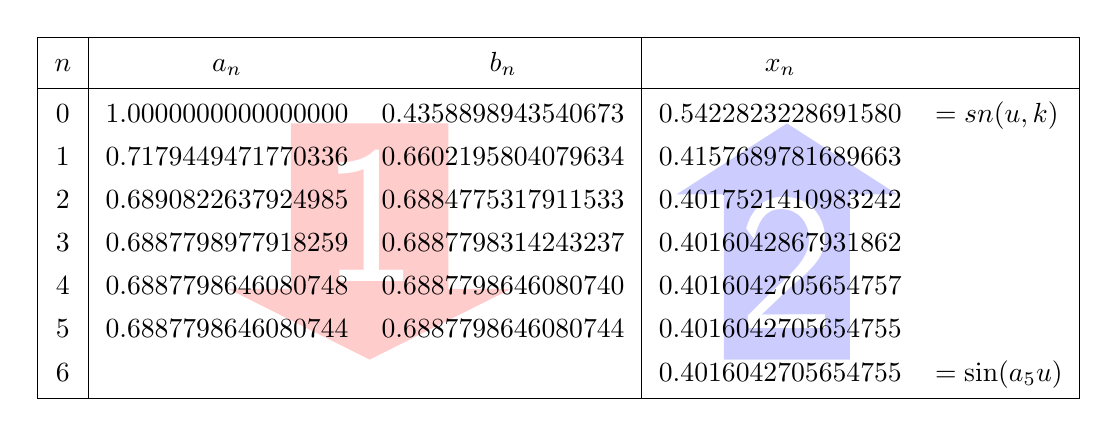
\begin{tikzpicture}[>=latex,thick]

\begin{scope}[xshift=-2.4cm,yshift=1.2cm]
\fill[color=red!20]
	(-1.0,0) -- (-1.0,-2.1) -- (-1.8,-2.1) -- (0,-3.0)
	-- (1.8,-2.1) -- (1.0,-2.1) -- (1.0,0) -- cycle;
\node[color=white] at (0,-1.2) [scale=7] {\sf 1};
\end{scope}

\begin{scope}[xshift=2.9cm,yshift=-1.8cm]
\fill[color=blue!20]
	(0.8,0) -- (0.8,2.1) -- (1.4,2.1) -- (0,3.0) -- (-1.4,2.1)
	-- (-0.8,2.1) -- (-0.8,0) -- cycle;
\node[color=white] at (0,1.2) [scale=7] {\sf 2};
\end{scope}

\node at (0,0) {
\begin{tabular}{|>{$}c<{$}|>{$}c<{$}>{$}c<{$}|>{$}c<{$}>{$}l<{$}|}
\hline
n & a_n                & b_n                  & x_n              &
\mathstrut\text{\vrule height12pt depth6pt width0pt}\\
\hline
0 & 1.0000000000000000 & 0.4358898943540673 & 0.5422823228691580 & = \operatorname{sn}(u,k)%
\mathstrut\text{\vrule height12pt depth0pt width0pt}\\
1 & 0.7179449471770336 & 0.6602195804079634 & 0.4157689781689663 & \mathstrut\\
2 & 0.6890822637924985 & 0.6884775317911533 & 0.4017521410983242 & \mathstrut\\
3 & 0.6887798977918259 & 0.6887798314243237 & 0.4016042867931862 & \mathstrut\\
4 & 0.6887798646080748 & 0.6887798646080740 & 0.4016042705654757 & \mathstrut\\
5 & 0.6887798646080744 & 0.6887798646080744 & 0.4016042705654755 & \mathstrut\\
6 &                    &                    & 0.4016042705654755 & = \sin(a_5u) 
\mathstrut\text{\vrule height0pt depth6pt width0pt}\\
\hline
\end{tabular}
};
\end{tikzpicture}
\caption{Berechnung von $\operatorname{sn}(u,k)$ für $u=0.6$ und $k=0.$2
mit Hilfe des arithmetisch-geo\-me\-tri\-schen Mittels.
In der ersten Phase des Algorithmus (rot) wird die Folge der arithmetischen
\index{Algorithmus!arithmetisch-geometrisches Mittel}%
und geometrischen Mittel berechnet, in der zweiten Phase die
Approximationen von $x_0=\operatorname{sn}(u,k)$.
Bei $n=5$ erreicht die Iteration des arithmetisch-geometrischen Mittels
Maschinengenauigkeit, was sich auch darin äussert, dass sich $x_5$ und
$x_6=\sin(a_5u)$ nicht unterscheiden.
\label{buch:elliptisch:agm:table:snberechnung}}
\end{table}
In Abschnitt~\ref{buch:elliptisch:subsection:agm} auf
Seite~\pageref{buch:elliptisch:subsubection:berechnung-fxk-agm}
wurde erklärt, wie das unvollständige elliptische Integral $F(x,k)$ mit 
Hilfe des arithmetisch-geometrischen Mittels berechnet werden kann.
\index{Algorithmus!arithmetisch-geometrisches Mittel}%
\index{arithmetisch-geometrisches Mittel!Algorithmus}%
Da $\operatorname{sn}^{-1}(x,k) = F(x,k)$ die Umkehrfunktion ist, kann
man den Algorithmus auch zur Berechnung von $\operatorname{sn}(u,k)$ 
verwenden.
Dazu geht man wie folgt vor:
\begin{enumerate}
\item
$k'=\sqrt{1-k^2}$.
\item
Berechne die Folgen des arithmetisch-geometrischen Mittels
$a_n$ und $b_n$ mit $a_0=1$ und $b_0=k'$, bis zum Folgenindex $N$,
bei dem ausreichende Konvergenz eintegreten ist.
\item
Setze $x_N = \sin(a_N \cdot u)$.
\item
Berechnet für absteigende $n=N-1,N-2,\dots$ die Folge $x_n$ mit Hilfe
der Rekursionsformel
\begin{equation}
x_{n}
=
\frac{2a_nx_{n+1}}{a_n+b_n+(a_n-b_n)x_{n+1}^2},
\label{buch:elliptisch:agm:xnrek}
\end{equation}
die aus \eqref{buch:elliptisch:agm:subst}
durch die Substitution $x_n = \sin t_n$ entsteht.
\item
Setze $\operatorname{sn}(u,k) = x_0$.
\end{enumerate}
Da die Formel \eqref{buch:elliptisch:agm:xnrek} nicht unter den
numerischen Stabilitätsproblemen leidet, die früher auf
Seite~\pageref{buch:elliptisch:agm:ellintegral-stabilitaet}
diskutiert wurden, ist die Berechnung stabil und sehr schnell.
Tabelle~\ref{buch:elliptisch:agm:table:snberechnung}
zeigt die Berechnung am Beispiel $u=0.6$ und $k=0.2$.

%
% Pole und Nullstellen der Jacobischen elliptischen Funktionen
%
\subsubsection{Pole und Nullstellen der Jacobischen elliptischen Funktionen}
\begin{figure}
\centering
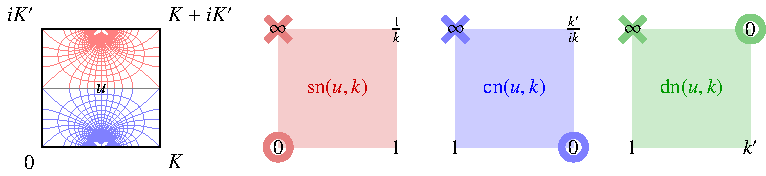
\includegraphics{chapters/110-elliptisch/images/ellpolnul.pdf}
\caption{Werte der grundlegenden Jacobischen elliptischen Funktionen
$\operatorname{sn}(u,k)$,
$\operatorname{cn}(u,k)$
und
$\operatorname{dn}(u,k)$
in den Ecken des Rechtecks mit Ecken $(0,0)$ und $(K,K+iK')$.
Links der Definitionsbereich, rechts die Werte der drei Funktionen.
Pole sind mit einem Kreuz ($\times$) bezeichnet, Nullstellen mit einem
Kreis ($\ocircle$).
\label{buch:elliptisch:fig:ellpolnul}}
\end{figure}
\begin{figure}
\centering
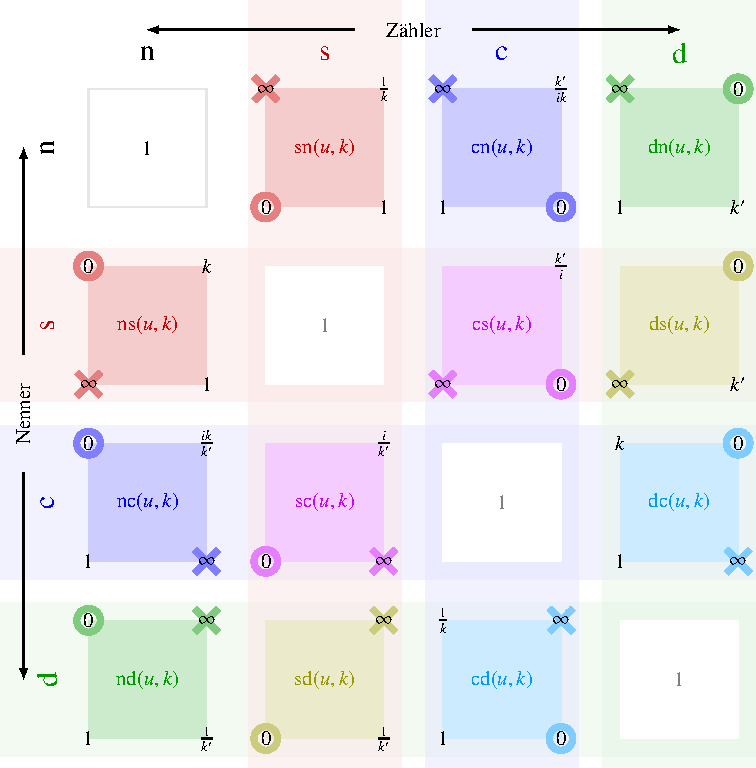
\includegraphics{chapters/110-elliptisch/images/ellall.pdf}
\caption{Pole und Nullstellen aller Jacobischen elliptischen Funktionen
mit den gleichen Darstellungskonventionen wie in
Abbildung~\ref{buch:elliptisch:fig:ellpolnul}
\label{buch:elliptisch:fig:ellall}}
\end{figure}
\begin{figure}
\centering
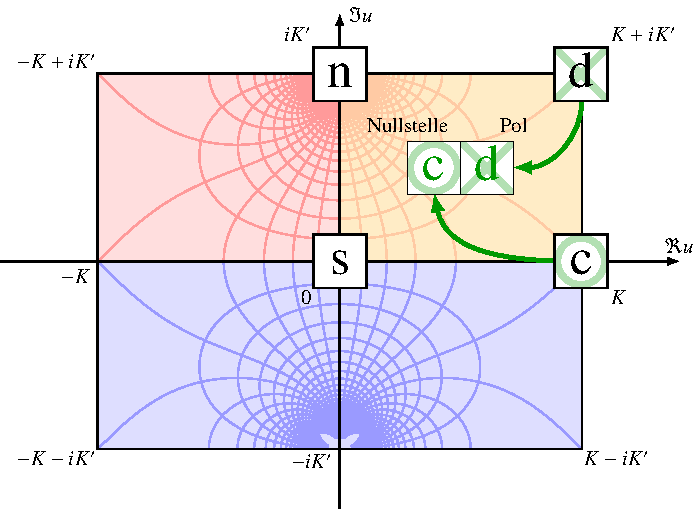
\includegraphics{chapters/110-elliptisch/images/ellselection.pdf}
\caption{Auswahl einer Jacobischen elliptischen Funktion mit bestimmten
Nullstellen und Polen.
Nullstellen und Pole können in jeder der vier Ecken des fundamentalen
Rechtecks (gelb, oberer rechter Viertel des Periodenrechtecks) liegen.
Der erste Buchstabe des Namens der gesuchten Funktion ist der Buchstabe
der Ecke der Nullstelle, der zweite Buchstabe ist der Buchstabe der
Ecke des Poles.
Im Beispiel die Funktion $\operatorname{cd}(u,k)$, welche eine
Nullstelle in $K$ hat und einen Pol in $K+iK'$.
\label{buch:elliptisch:fig:selectell}}
\end{figure}
Für die Funktion $y=\operatorname{sn}(u,k)$ erfüllt die Differentialgleichung
\[
\frac{dy}{du}
=
\sqrt{(1-y^2)(1-k^2y^2)},
\]
welche mit dem unbestimmten Integral
\begin{equation}
u + C = \int\frac{dy}{\sqrt{(1-y^2)(1-k^2y^2)}}
\label{buch:elliptisch:eqn:uyintegral}
\end{equation}
gelöst werden kann.
Der Wertebereich des Integrals in \eqref{buch:elliptisch:eqn:uyintegral}
wurde bereits in
Abschnitt~\ref{buch:elliptisch:subsection:unvollstintegral}
auf Seite~\pageref{buch:elliptische:subsubsection:wertebereich}
diskutiert.
Daraus können jetzt Nullstellen und Pole der Funktion $\operatorname{sn}(u,k)$
und mit Hilfe von Tabelle~\ref{buch:elliptisch:fig:jacobi-relationen}
auch für $\operatorname{cn}(u,k)$ und $\operatorname{dn}(u,k)$
abgelesen werden:
\begin{equation}
\begin{aligned}
\operatorname{sn}(0,k)&=0
&&\qquad&
\operatorname{cn}(0,k)&=1
&&\qquad&
\operatorname{dn}(0,k)&=1
\\
\operatorname{sn}(iK',k)&=\infty
&&\qquad&
\operatorname{cn}(iK',k)&=\infty
&&\qquad&
\operatorname{dn}(iK',k)&=\infty
\\
\operatorname{sn}(K,k)&=1
&&\qquad&
\operatorname{cn}(K,k)&=0
&&\qquad&
\operatorname{dn}(K,k)&=k'
\\
\operatorname{sn}(K+iK',k)&=\frac{1}{k}
&&\qquad&
\operatorname{cn}(K+iK',k)&=\frac{k'}{ik}
&&\qquad&
\operatorname{dn}(K+iK',k)&=0.
\end{aligned}
\label{buch:elliptische:eqn:eckwerte}
\end{equation}
Abbildung~\ref{buch:elliptisch:fig:ellpolnul} zeigt diese Werte
an einer schematischen Darstellung des Definitionsbereiches auf.
Daraus lassen sich jetzt auch die Werte der abgeleiteten Jacobischen
elliptischen Funktionen ablesen, Pole und Nullstellen sind in
Abbildung~\ref{buch:elliptisch:fig:ellall}
zusammengestellt.





%
% Differentialgleichung des anharmonischen Oszillators
%
\subsubsection{Differentialgleichung des anharmonischen Oszillators}
Wir möchten die nichtlineare Differentialgleichung
\index{Differentialgleichung!das anharmonischen Oszillators}%
\begin{equation}
\biggl(
\frac{dx}{dt}
\biggr)^2
=
Ax^4+Bx^2 + C
\label{buch:elliptisch:eqn:anhdgl}
\end{equation}
mit Hilfe elliptischer Funktionen lösen.
Wir nehmen also an, dass die gesuchte Lösung eine Funktion der Form
\begin{equation}
x(t) = a\operatorname{zn}(bt,k)
\label{buch:elliptisch:eqn:loesungsansatz}
\end{equation}
ist.
Die erste Ableitung von $x(t)$ ist
\[
\dot{x}(t) 
=
a\operatorname{zn}'(bt,k).
\]

Indem wir diesen Lösungsansatz in die
Differentialgleichung~\eqref{buch:elliptisch:eqn:anhdgl}
einsetzen, erhalten wir
\begin{equation}
a^2b^2 \operatorname{zn}'(bt,k)^2
=
a^4A\operatorname{zn}(bt,k)^4
+
a^2B\operatorname{zn}(bt,k)^2
+C
\label{buch:elliptisch:eqn:dglx}
\end{equation}
Andererseits wissen wir, dass $\operatorname{zn}(u,k)$ einer
Differentialgleichung der Form~\eqref{buch:elliptisch:eqn:1storderdglell}
erfüllt.
Wenn wir \eqref{buch:elliptisch:eqn:dglx} durch $a^2b^2$ teilen, können wir
die rechte Seite von \eqref{buch:elliptisch:eqn:dglx} mit der rechten
Seite von \eqref{buch:elliptisch:eqn:1storderdglell} vergleichen:
\[
\frac{a^2A}{b^2}\operatorname{zn}(bt,k)^4
+
\frac{B}{b^2}\operatorname{zn}(bt,k)^2
+\frac{C}{a^2b^2}
=
\alpha\operatorname{zn}(bt,k)^4
+
\beta\operatorname{zn}(bt,k)^2
+
\gamma\operatorname{zn}(bt,k).
\]
Daraus ergeben sich die Gleichungen
\begin{align}
\alpha &= \frac{a^2A}{b^2},
&
\beta &= \frac{B}{b^2}
&&\text{und}
&
\gamma &= \frac{C}{a^2b^2}
\label{buch:elliptisch:eqn:koeffvergl}
\intertext{oder aufgelöst nach den Koeffizienten der ursprünglichen
Differentialgleichung}
A&=\frac{\alpha b^2}{a^2}
&
B&=\beta b^2
&&\text{und}&
C &= \gamma a^2b^2
\label{buch:elliptisch:eqn:koeffABC}
\end{align}
für die Koeffizienten der Differentialgleichung der zu verwendenden
Funktion.

Man beachte, dass nach \eqref{buch:elliptisch:eqn:koeffvergl} die 
Koeffizienten $A$, $B$ und $C$ die gleichen Vorzeichen haben wie
$\alpha$, $\beta$ und $\gamma$, da in 
\eqref{buch:elliptisch:eqn:koeffvergl} nur mit Quadraten multipliziert
wird, die immer positiv sind.
Diese Vorzeichen bestimmen, welche der Funktionen gewählt werden muss.

In den Differentialgleichungen für die elliptischen Funktionen gibt
es nur den Parameter $k$, der angepasst werden kann.
Es folgt, dass die Gleichungen
\eqref{buch:elliptisch:eqn:koeffvergl} 
auch $a$ und $b$ bestimmen.
Zum Beispiel folgt aus der letzten Gleichung, dass
\[
b = \pm\sqrt{\frac{B}{\beta}}.
\]
Damit folgt dann aus der zweiten
\[
a=\pm\sqrt{\frac{\beta C}{\gamma B}}.
\]
Die verbleibende Gleichung legt $k$ fest.
Das folgende Beispiel illustriert das Vorgehen am Beispiel einer
Gleichung, die Lösungsfunktion $\operatorname{sn}(u,k)$ verlangt.

\begin{beispiel}
Wir nehmen an, dass die Vorzeichen von $A$, $B$ und $C$ gemäss
Tabelle~\ref{buch:elliptisch:tabelle:loesungsfunktionen} verlangen,
dass die Funktion $\operatorname{sn}(u,k)$ für die Lösung verwendet
werden muss.
Die Tabelle sagt dann auch, dass 
$\alpha=k^2$, $\beta=1$ und $\gamma=1$ gewählt werden müssen.
Aus dem Koeffizientenvergleich~\eqref{buch:elliptisch:eqn:koeffvergl}
folgt der Reihe nach
\begin{align*}
b&=\pm \sqrt{B}
\\
a&=\pm \sqrt{\frac{C}{B}}
\\
k^2
&=
\frac{AC}{B^2}.
\end{align*}
Man beachte, dass man $k^2$ durch Einsetzen von
\eqref{buch:elliptisch:eqn:koeffABC}
auch direkt aus den Koeffizienten $\alpha$, $\beta$ und $\gamma$
erhalten kann, nämlich
\[
\frac{AC}{B^2}
=
\frac{\frac{\alpha b^2}{a^2} \gamma a^2b^2}{\beta^2 b^4}
=
\frac{\alpha\gamma}{\beta^2}.
\qedhere
\]
\end{beispiel}

Da alle Parameter im 
Lösungsansatz~\eqref{buch:elliptisch:eqn:loesungsansatz} bereits
festgelegt sind, stellt sich die Frage, woher man einen weiteren
Parameter nehmen kann, mit dem Anfangsbedingungen erfüllen kann.
Die Differentialgleichung~\eqref{buch:elliptisch:eqn:anhdgl} ist
autonom, die Koeffizienten der rechten Seite der Differentialgleichung
sind nicht von der Zeit abhängig. 
Damit ist eine zeitverschobene Funktion $x(t-t_0)$ ebenfalls eine
Lösung der Differentialgleichung.
Die allgmeine Lösung der 
Differentialgleichung~\eqref{buch:elliptisch:eqn:anhdgl} hat
also die Form
\[
x(t) = a\operatorname{zn}(b(t-t_0)),
\]
wobei die Funktion $\operatorname{zn}(u,k)$ auf Grund der Vorzeichen
von $A$, $B$ und $C$ gewählt werden müssen.

Die Übungsaufgaben~\ref{buch:elliptisch:aufgabe:1} ist als
Lernaufgabe konzipiert, mit der die Lösung der Differentialgleichung
des harmonischen Oszillators beispielhaft durchgearbeitet
werden kann.

%
% 23-mathpendel.tex -- Das mathematische Pendel
%
% (c) 2022 Prof Dr Andreas Müller, OST Ostschweizer Fachhochschule
%

\subsection{Das mathematische Pendel
\label{buch:elliptisch:subsection:mathpendel}}
\begin{figure}
\centering
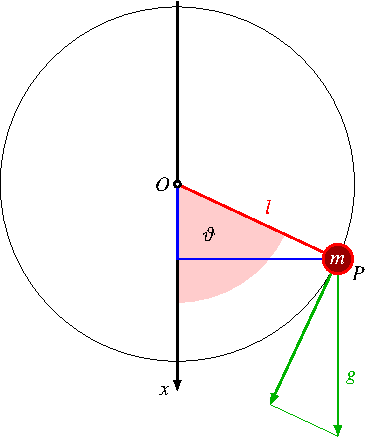
\includegraphics{chapters/110-elliptisch/images/pendel.pdf}
\caption{Mathematisches Pendel
\label{buch:elliptisch:fig:mathpendel}}
\end{figure}
Das in Abbildung~\ref{buch:elliptisch:fig:mathpendel} dargestellte
Mathematische Pendel besteht aus einem Massepunkt der Masse $m$
im Punkt $P$,
der über eine masselose Stange der Länge $l$ mit dem Drehpunkt $O$
verbunden ist.
Das Pendel bewegt sich unter dem Einfluss der Schwerebeschleunigung $g$.

Das Trägheitsmoment des Massepunktes um den Drehpunkt $O$ ist
\(
I=ml^2
\).
Das Drehmoment der Schwerkraft ist
\(M=gl\sin\vartheta\).
Die Bewegungsgleichung wird daher
\[
\begin{aligned}
\frac{d}{dt} I\dot{\vartheta}
&=
M
=
gl\sin\vartheta
\\
ml^2\ddot{\vartheta}
&=
gl\sin\vartheta
&&\Rightarrow&
\ddot{\vartheta}
&=\frac{g}{l}\sin\vartheta.
\end{aligned}
\]
Dies ist eine nichtlineare Differentialgleichung zweiter Ordnung, die
wir nicht unmittelbar mit den Differentialgleichungen erster Ordnung
der elliptischen Funktionen vergleichen können.

Die Differentialgleichungen erster Ordnung der elliptischen Funktionen
enthalten das Quadrat der ersten Ableitung.
In unserem Fall entspricht das einer Gleichung, die $\dot{\vartheta}^2$
enthält.
Der Energieerhaltungssatz kann uns eine solche Gleichung geben.
Die Summe von kinetischer und potentieller Energie muss konstant sein.
Dies führt auf
\begin{equation}
E_{\text{kinetisch}}
+
E_{\text{potentiell}}
=
\frac12I\dot{\vartheta}^2
+
mgl(1-\cos\vartheta)
=
\frac12ml^2\dot{\vartheta}^2
+
mgl(1-\cos\vartheta)
=
E.
\label{buch:elliptisch:mathpendel:energiegleichung}
\end{equation}
Durch Auflösen nach $\dot{\vartheta}$ kann man jetzt die
Differentialgleichung
\[
\dot{\vartheta}^2
=
-
\frac{2g}{l}(1-\cos\vartheta)
+\frac{2E}{ml^2}
\]
finden.
In erster Näherung, d.h. wenn man die rechte Seite bis zu vierten
Potenzen in eine Taylor-Reihe in $\vartheta$ entwickelt,  ist dies
tatsächlich eine Differentialgleichung der Art, wie wir sie für
elliptische Funktionen gefunden haben, wir möchten aber eine exakte
Lösung konstruieren.

Die maximale Energie für eine Bewegung, bei der sich das Pendel gerade
über den höchsten Punkt hinweg zu bewegen vermag, ist 
$E=2lmg$.
Falls $E<2mgl$ ist, erwarten wir Schwingungslösungen, bei denen 
der Winkel $\vartheta$ immer im offenen Interval $(-\pi,\pi)$
bleibt.
Für $E>2mgl$ wird sich das Pendel im Kreis bewegen, für sehr grosse
Energie ist die kinetische Energie dominant, die Verlangsamung im
höchsten Punkt wird immer weniger ausgeprägt sein.


%
% Koordinatentransformation auf elliptische Funktionen
%
\subsubsection{Koordinatentransformation auf elliptische Funktionen}
Wir verwenden als neue Variable 
\begin{align}
y
&=
\sin\frac{\vartheta}2
&&\Rightarrow&
\cos^2\frac{\vartheta}2
&=
1-y^2.
\label{buch:elliptisch:mathpendel:ydef}
\intertext{Die Ableitung ist}
\dot{y}
&=
\frac12\cos\frac{\vartheta}{2}\cdot \dot{\vartheta}
&&\Rightarrow&
\dot{y}^2
&=
\frac14\cos^2\frac{\vartheta}2\cdot\dot{\vartheta}^2.
\label{buch:elliptisch:mathpendel:yabl}
\intertext{%
Man beachte, dass die Koordinate senkrecht zur $x$-Achse in 
Abbildung~\ref{buch:elliptisch:fig:mathpendel} die Auslenkung
$l\sin\vartheta$ ist, $y$ ist also nicht die Auslenkung senkrecht
zur $x$-Achse!
Aus den Halbwinkelformeln finden wir ausserdem
}
\cos\vartheta
&=
1-2\sin^2 \frac{\vartheta}2
=
1-2y^2
&&\Rightarrow&
1-\cos\vartheta
&=
2y^2.
\label{buch:elliptisch:mathpendel:halbwinkel}
\end{align}
Die Grösse $1-\cos\vartheta$ haben wir in der Energiegleichung
\eqref{buch:elliptisch:mathpendel:energiegleichung}
bereits angetroffen.

Die Identitäten 
\eqref{buch:elliptisch:mathpendel:halbwinkel}
%und
%\eqref{buch:elliptisch:mathpendel:ydef}
können wir jetzt in die
Energiegleichung~\eqref{buch:elliptisch:mathpendel:energiegleichung}
einsetzen und erhalten
\begin{align}
\frac12ml^2\dot{\vartheta}^2 + 2mgly^2
&=
E
\intertext{und nach Division durch $2ml^2$}
\frac14 \dot{\vartheta}^2
&=
\frac{E}{2ml^2} - \frac{g}{l}y^2.
\label{buch:elliptisch:mathpendel:thetadgl}
\end{align}
%Der konstante Term auf der rechten Seite ist grösser oder kleiner als
%$1$ je nachdem, ob das Pendel sich im Kreis bewegt oder nicht.
Durch Multiplizieren mit der rechten Gleichung von
\eqref{buch:elliptisch:mathpendel:ydef}
erhalten wir auf der linken Seite einen Ausdruck, den wir
mit Hilfe von \eqref{buch:elliptisch:mathpendel:yabl}
als Funktion von $\dot{y}$ ausdrücken können.
Wir erhalten
\begin{align}
\underbrace{\frac14
\cos^2\frac{\vartheta}2
\cdot
\dot{\vartheta}^2}_{\displaystyle=\dot{y}^2}
&=
(1-y^2)
\biggl(\frac{E}{2ml^2} -\frac{g}{l}y^2\biggr)
\notag
\\
\dot{y}^2
&=
(1-y^2)
\biggl(\frac{E}{2ml^2} -\frac{g}{l}y^2\biggr).
\label{buch:elliptisch:mathpendel:ydgl}
\end{align}
Die letzte Gleichung hat die Form einer Differentialgleichung
für elliptische Funktionen.
Welche Funktion verwendet werden muss, hängt von der relativen
Grösse der Koeffizienten in der zweiten Klammer ab.

%
% Zeittransformation zur Elimination des konstanten Faktors
%
\subsubsection{Zeittransformation}
Die Gleichung~\eqref{buch:elliptisch:mathpendel:ydgl} kann auch in
die Form
\begin{equation}
\frac{2ml^2}{E}\dot{y}^2
=
(1-y^2)\biggl(1-\frac{2mgl}{E}y^2\biggr)
\label{buch:elliptisch:mathpendel:ydgl2}
\end{equation}
gebracht werden.
Der konstante Faktor auf der linken Seite kann wie in der Diskussion
des anharmonischen Oszillators durch eine lineare
Transformation der Zeit zum Verschwinden gebracht werden.
Dazu setzt man $z(t) = y(bt)$ und bekommt
\[
\frac{d}{dt}z(t)
=
\frac{d}{dt}y(bt) \frac{d\,bt}{dt}
=
b\,\dot{y}(bt).
\]
Die Zeit muss also mit dem Faktor $\sqrt{2ml^2/E}$ skaliert werden.

%
% Nullstellen der rechten Seite der Differentialgleichung
%
\subsubsection{Nullstellen der rechten Seite}
Die rechte Seite von \eqref{buch:elliptisch:mathpendel:ydgl2}
hat die beiden Nullstellen $1$ und
\begin{equation}
y_0=\sqrt{\frac{E}{2mgl}}. 
\label{buch:elliptisch:mathpendel:y0}
\end{equation}
Die Differentialgleichung kann damit als
\begin{equation}
\dot{y}^2
=
(1-y^2)\biggl(1-\frac{1}{y_0^2}y^2\biggr)
\label{buch:elliptisch:mathpendel:y0dgl}
\end{equation}
geschrieben werden.
Da die linke Seite $\ge 0$ sein muss, muss 
\(
y\le \min(1,y_0)
\)
sein.
Damit ergeben sich zwei Fälle.
Wenn $y_0<1$ ist, dann schwingt das Pendel.
Der Fall $y_0>1$ entspricht einer Bewegung, bei der das Pendel
um den Punkt $O$ rotiert.
In den folgenden zwei Abschnitten werden die beiden Fälle ausführlicher
diskutiert.


\begin{figure}
\centering
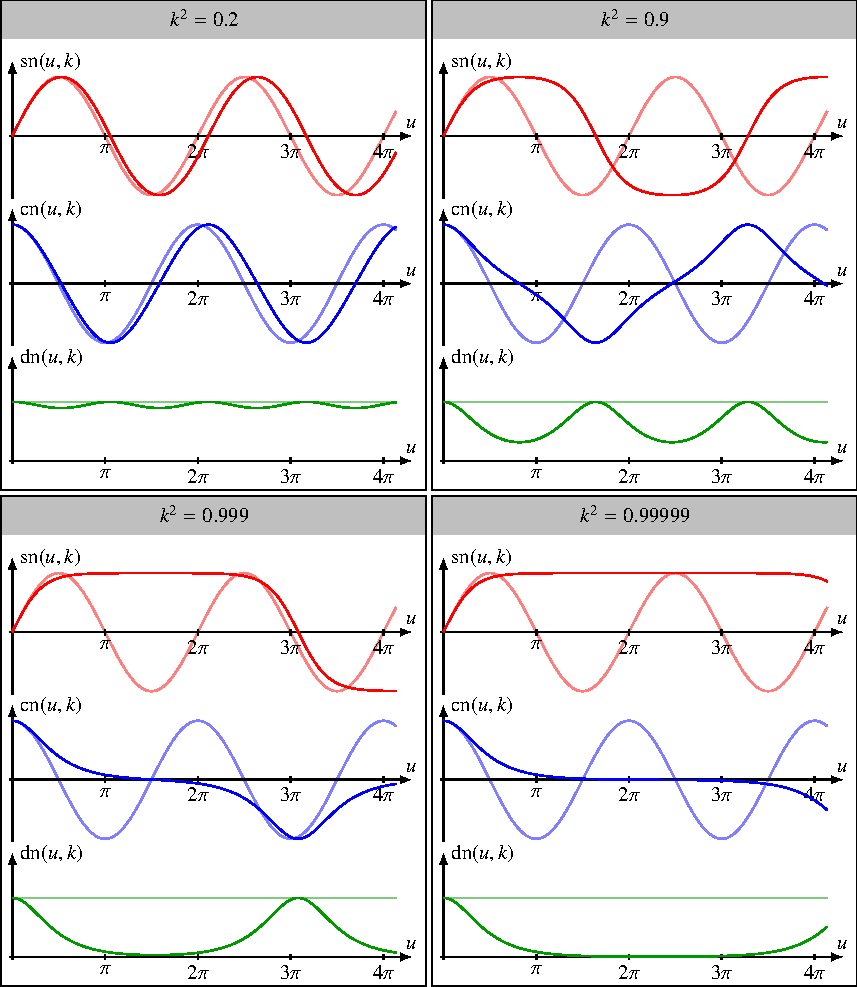
\includegraphics[width=\textwidth]{chapters/110-elliptisch/images/jacobiplots.pdf}
\caption{%
Abhängigkeit der elliptischen Funktionen von $u$ für
verschiedene Werte von $k^2=m$.
Für $m=0$ ist $\operatorname{sn}(u,0)=\sin u$, 
$\operatorname{cn}(u,0)=\cos u$ und $\operatorname{dn}(u,0)=1$, diese
sind in allen Plots in einer helleren Farbe eingezeichnet.
Für kleine Werte von $m$ weichen die elliptischen Funktionen nur wenig
von den trigonometrischen Funktionen ab,
es ist aber klar erkennbar, dass die anharmonischen Terme in der
Differentialgleichung die Periode mit steigender Amplitude verlängern.
Sehr grosse Werte von $m$ nahe bei $1$ entsprechen der Situation, dass
die Energie des Pendels fast ausreicht, dass es den höchsten Punkt
erreichen kann, was es für $m$ macht.
\label{buch:elliptisch:fig:jacobiplots}}
\end{figure}

\subsubsection{Der Fall $E>2mgl$}
In diesem Fall ist die zweite Nullstelle $y_0>1$ oder $1/y_0^2 < 1$.
Die Differentialgleichung~\eqref{buch:elliptisch:mathpendel:y0dgl}
sieht ganz ähnlich aus wie die Differentialgleichung der
Funktion $\operatorname{sn}(u,k)$, tatsächlich wird sie zur
Differentialgleichung von $\operatorname{sn}(u,k)$ wenn man
\[
k^2
=
1/y_0^2
=
\frac{2mgl}{E}
\]
wählt.
In diesem Fall ist also $y=\operatorname{sn}(u,1/y_0)$ eine Lösung
der Differentialgleichung, wobei $u$ eine lineare Funktion der Zeit
ist.

Wenn $y_0 \gg 1$ ist, dann ist $k\approx 0$ und die Bewegung ist
entspricht einer gleichförmigen Kreisbewegung.
Je näher $y_0$ an $1$ liegt, desto näher an $1$ ist auch $k$ und
desto grösser wird die Verlangsamung der Bewgung in der Nähe des
Scheitels, das Pendel verweilt sehr lange.
Dies äussert sich in Abbildung~\ref{buch:elliptisch:fig:jacobiplots}
durch die lange Verweildauer der Funktion nahe der Extrema.

%
% Der Fall E < 2mgl
%
\subsubsection{Der Fall $E<2mgl$}
In diesem Fall ist $y_0<1$ und die
Differentialgleichung~\eqref{buch:elliptisch:mathpendel:y0dgl}
sieht zwar immer noch wie eine Differentialgleichung für
$\operatorname{sn}(u,k)$ aus, aber die Lage der Nullstellen
der rechten Seite ist verkehrt.
Indem wir $y=y_0z$ schreiben, erhalten wir 
\begin{equation}
\dot{y}^2
=
y_0^2 \dot{z}^2
=
(1-y_0^2z^2)(1-z^2).
\end{equation}
Wieder kann durch eine lineare Transformation der Zeit der Faktor $y_0^2$
auf der linken Seite zum Verschwinden gebracht werden, es bleibt
die Differentialgleichung der Funktion $\operatorname{sn}(u,k)$
mit $k=y_0$.
Daraus liest man ab, dass $y_0\operatorname{sn}(u,k)$ die Bewegung
des Pendels im oszillatorischen Fall beschreibt, wobei $u$ wieder
eine lineare Funktion der Zeit ist.

Wenn $y_0\ll 1$ ist, dann ist auch $k$ sehr klein und die lineare
Näherung ist sehr gut, das Pendel verhält sich wie ein harmonischer
Oszillator mit einer Sinus-Schwingung als Lösung.
Für $y_0=k$ nahe an $1$ dagegen erreicht die Schwingung fast den
die maximale Höhe und wird dort sehr langsam.
Dies äussert sich in Abbildung~
Dies äussert sich in Abbildung~\ref{buch:elliptisch:fig:jacobiplots}
wiederum durch die lange Verweildauer der Funktion nahe der Extrema.



